\chapter{ĐÁNH GIÁ CHẤT LƯỢNG HỆ THỐNG ĐIỀU KHIỂN}
\[
    G(s) = \frac{4.85}{s^2 + 53.51}
\]
\section{Các tiêu chuẩn về xác lập}
Hàm truyền vòng kín:
\[
    T(s) = \frac{G(s)}{1+G(s)} = \frac{4.85}{s^2 + 58.36}
\]
Xét với đầu vào bậc (step input, $R(s)=\frac{1}{s}$), sai số xác lập được tính bằng:
\[
e_{xl} = \lim_{s \to 0} \frac{s \cdot R(s)}{1 + G(s)} 
= \lim_{s \to 0} \frac{1}{1 + k_p} \approx 0{,}92
\]
\begin{center}
    Với $k_p$  là hệ số vị trí, $k_p = \lim_{s \to 0} G(s) \approx 0.09$ 
\end{center}
\textbf{Khảo sát hệ thống là bậc 2}
\begin{figure}[H]
    \centering
    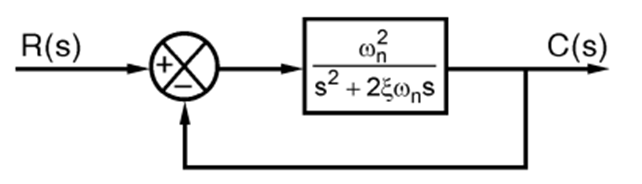
\includegraphics[width=0.8\textwidth]{pictures/closeloop.png}
\end{figure}

Hàm truyền hệ dao động bậc 2:
\[
    G_2(s) = \frac{K\omega^2}{s^2+2\zeta \omega s + \omega^2}
\]
Đáp ứng quá độ:
\[
    C(s) = R(s)\cdot G_2(s) = \frac{1}{s}\cdot \frac{K\omega^2}{s^2+2\zeta \omega s + \omega^2}
\]
$\Rightarrow$ Laplace ngược: 
\[
    c(t) = K\{1-\frac{e^{-\zeta \omega_n t}}{\sqrt{1-\zeta^2}}\cdot sin[(\omega_n\sqrt{1-\zeta^2})\cdot t+\theta] \}
\]
Qua đó ta thấy hệ dao động không giảm chấn với $\zeta = 0$.\\
Hệ dao động bậc 2 có 2 cặp cực phức: $p_{1,2} = \pm j\,7{,}639$ \\

\textbf{Từ đó xác định các thông số cơ bản }
\begin{itemize}
    \item Tần số tự nhiên: $\omega_n = 7{,}639$
    \item Hệ số giảm chấn: $\zeta = 0$
    \item Thời gian đạt đỉnh: $T_p = \frac{\pi}{\omega_n \sqrt{1 - \zeta^2}} = 0{,}411s$
    \item Độ vọt lố: $\text{POT} = e^{\frac{-\zeta \pi}{1-\zeta^2}} \cdot 100 = 100\%$
    \item Thời gian xác lập: Với tiêu chuẩn 2\% $\Rightarrow T_p = \frac{4}{\zeta \omega_n} \rightarrow \infty$
    \item Đáp ứng quá độ: $C(s) = R(s) \cdot T(s) = \frac{1}{s} \cdot \frac{4{,}85}{s^2 + 58{,}36}$
\end{itemize}
\[
\Rightarrow c(t) = \frac{4.85}{7.639^2} \left[1 - \sin(7.639 \cdot t + \frac{\pi}{2})\right] = 0.083 - 0.083 \cos(7.639 \cdot t)
\]
\begin{figure}[H]
    \centering
    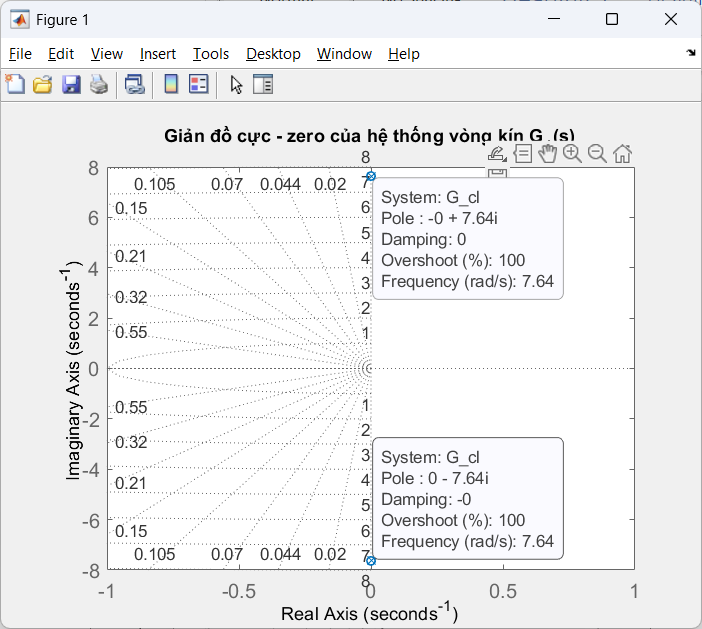
\includegraphics[width=0.8\textwidth]{pictures/poleszeros.png}
\end{figure}
\begin{figure}[H]
    \centering
    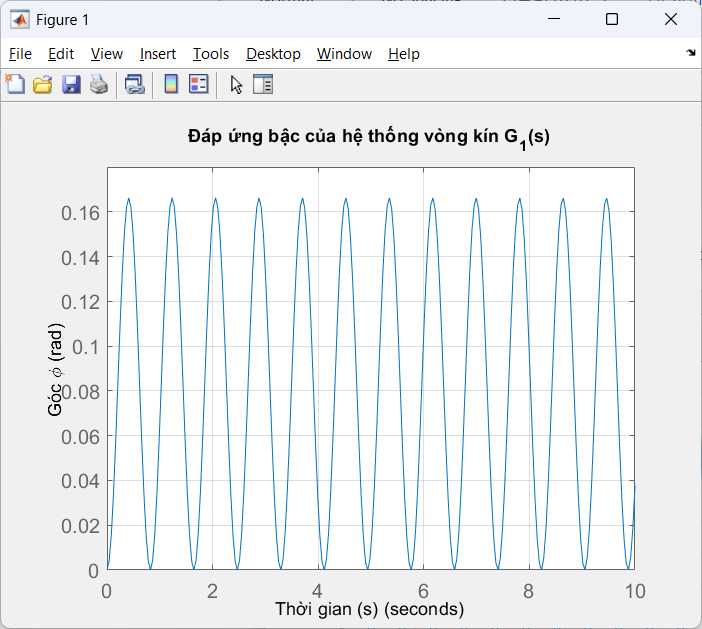
\includegraphics[width=0.8\textwidth]{pictures/step.png}
\end{figure}
\textbf{Nhận xét:} Đáp ứng quá độ của khâu dao động bậc 2 có dạng dao động với biên độ giảm dần.
Do $\zeta = 0$, đáp ứng của hệ là dao động không suy giảm với tần số tự nhiên $\omega_n = 7.639$.